\subsection*{Άσκηση 1}

Εξετάστε αν για κάθε απλό συνεκτικό $d$-κανονικό γράφημα $G$, κάθε κορυφή είναι κεντρική
και απόκεντρη. Αν ισχύει αποδείξτε το, αλλιώς δώστε ένα αντιπαράδειγμα.

\subsubsection*{Λύση}

Δεν ισχύει, παρατίθεται αντιπαράδειγμα για 3-κανονικό γράφημα:

\begin{center}
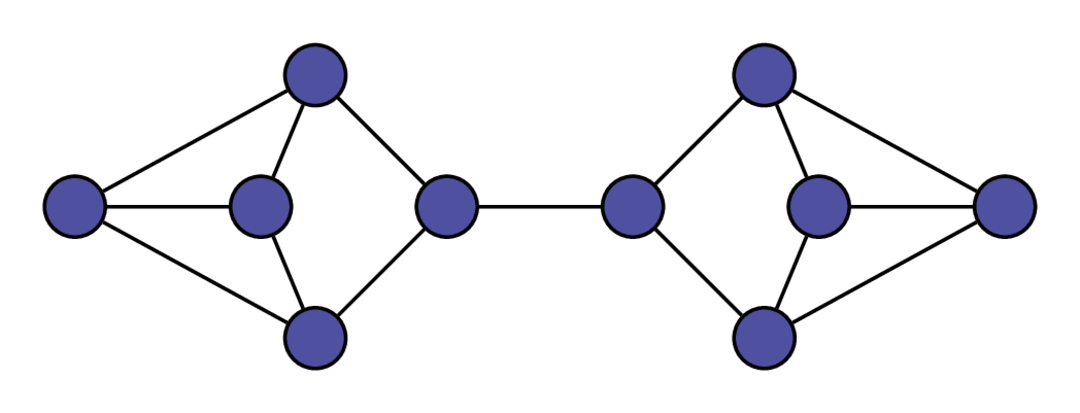
\includegraphics[height=4cm, width=10cm]{exercise1/diagrams/d1.png}
\end{center}

